%----------------------------------------------------------
% Capítulo 3 – Desarrollo
%----------------------------------------------------------

%----------------------------------------------------------
\section{Base de datos}
%----------------------------------------------------------

\begin{large}

Para esta plataforma, la base de datos se implementó íntegramente en Firestore, aprovechando su modelo NoSQL en tiempo real y su escalabilidad automática. A continuación se describen los pasos clave:

\end{large}

\subsection{Configuración inicial en Firebase}

\begin{large}

En primer lugar, se creó un proyecto en la consola de Firebase y se habilitaron los servicios de Firestore y Authentication. Dentro de Firestore, se generó la colección raíz \texttt{businesses}, donde cada documento tiene un identificador único (\texttt{businessId}). De forma automática, Firestore asigna una referencia a cada colección y subcolección cuando se insertan documentos por primera vez desde los clientes.

Para conectar la aplicación iOS, se descargó el archivo \texttt{GoogleService-Info.plist} desde la consola de Firebase y se añadió al directorio principal del proyecto Xcode. En el caso del portal web, se obtuvo el objeto de configuración (API key, project ID, etc.), se guardó en un archivo \texttt{.env} y se cargó desde un archivo \texttt{config.ts} bajo \texttt{/src/firebase}.

\end{large}

\subsection{Reglas de seguridad de Firestore}

\begin{large}

Para garantizar que solo los usuarios autorizados accedieran a la información, se definieron reglas en el panel de Firestore. Un extracto de las reglas más relevantes es:

\begin{lstlisting}[language={}, caption={Reglas de seguridad de Firestore}]
rules_version = '2';
service cloud.firestore {
  match /databases/{database}/documents {
    
    // Raíz de negocios: controlamos creación/lectura/actualización/borrado a nivel de negocio
    match /businesses/{businessId} {
      // Cualquiera autenticado puede leer la información de un negocio
      allow read: if request.auth != null;
      // Cualquiera autenticado puede crear un nuevo negocio
      allow create: if request.auth != null;
      // Solo un admin (claim role == "admin") puede modificar o borrar un negocio
      allow update, delete: if request.auth.token.role == 'admin';
      
      // Subcolección de empleados: solo admins pueden gestionar empleados
      match /employees/{employeeId} {
        allow read: if request.auth != null;
        allow create, update, delete: if request.auth.token.role == 'admin';
      }
      
      // Subcolección de clientes: 
      //   - cualquiera autenticado ve datos de clientes
      //   - un admin o el propio cliente (uid == userClientId) puede crear/editar/borrar
      match /clients/{clientId} {
        allow read: if request.auth != null;
        allow create: if request.auth.token.role == 'admin';
        allow update, delete: if request.auth.token.role == 'admin'
                              || request.auth.uid == resource.data.userClientId;
      }
      
      // Subcolección de facturas:
      //   - cualquiera autenticado puede leer
      //   - crear: admin o empleado que firma la factura (employeeId en request.resource.data)
      //   - actualizar: admin o empleado que creó la factura (employeeId en el dato existente)
      //   - borrar: solo admin
      match /invoices/{invoiceId} {
        allow read: if request.auth != null;
        allow create: if request.auth.token.role == 'admin'
                      || request.auth.uid == request.resource.data.employeeId;
        allow update: if request.auth.token.role == 'admin'
                      || request.auth.uid == resource.data.employeeId;
        allow delete: if request.auth.token.role == 'admin';
        
        // Dentro de cada factura, la subcolección de líneas de producto:
        //   - cualquiera autenticado puede leer
        //   - solo el admin puede escribir/borrar
        match /productsStack/{productStackId} {
          allow read: if request.auth != null;
          allow create, update, delete: if request.auth.token.role == 'admin';
        }
      }
      
      // Subcolección de productos: 
      //   - cualquiera autenticado puede leer
      //   - solo admin puede escribir/borrar
      match /products/{productId} {
        allow read: if request.auth != null;
        allow create, update, delete: if request.auth.token.role == 'admin';
      }
    }
    
  }
}
\end{lstlisting}

Con estas reglas, solo el administrador (rol \texttt{admin}) puede crear o eliminar facturas y productos, y cada empleado (rol \texttt{employee}) puede crear o actualizar facturas que él mismo genere. Los clientes solo acceden a sus propios documentos, y todas las operaciones requieren un usuario autenticado (\texttt{request.auth != null}), lo que cumple con los requisitos de seguridad y protección de datos.

\end{large}

%----------------------------------------------------------
\section{Implementación iOS}
%----------------------------------------------------------

\begin{large}

En esta sección profundizamos en la aplicación iOS, donde se dedicaron la mayoría de las horas de desarrollo. Partimos desde cero, aprendiendo Swift y SwiftUI, y construimos la app siguiendo el patrón MVVM para separar responsabilidades y lograr un código más mantenible.

\end{large}

\subsection{Configuración del proyecto y conexión a Firebase}

\begin{large}

Para iniciar el proyecto, se utilizó Xcode 16.3 con la plantilla de SwiftUI. Los pasos fueron:

\begin{enumerate}
  \item En Xcode, crear un nuevo proyecto seleccionando \emph{App} y, como lenguaje, \textbf{Swift} con interfaz \textbf{SwiftUI}.
  \item Descargar \texttt{GoogleService-Info.plist} desde la consola de Firebase y arrastrarlo al grupo raíz del proyecto en Xcode. Asegurarse de marcar la opción de agregarlo a todos los targets.
  \item Instalar el paquete oficial de Firebase mediante Swift Package Manager (\emph{File → Add Packages…}), usando la URL \url{https://github.com/firebase/firebase-ios-sdk.git}.
  \item En el archivo \texttt{QuickBillApp.swift}, inicializar Firebase antes de cargar la escena principal:
    \begin{lstlisting}[language={swift}, caption={Inicialización de Firebase en QuickBillApp.swift}]
    import SwiftUI
    import FirebaseCore
    
    @main
    struct QuickBillApp: App {
        @StateObject private var auth = AuthViewModel()
        @AppStorage("appLanguage") private var appLanguage: String = AppLanguage.english.rawValue
        
        init() {
            FirebaseApp.configure()
        }
        
        var body: some Scene {
            WindowGroup {
                if auth.isSignedIn {
                    MainTabView()
                } else {
                    StartView()
                }
            }
            .environmentObject(auth)
            .environment(\.locale, Locale(identifier: appLanguage))
        }
    }
    \end{lstlisting}
  \item Configurar en la consola de Firebase el dominio de la app, activando Authentication con correo/contraseña.
\end{enumerate}

Con estos pasos, la aplicación iOS ya está conectada a Firebase y lista para consumir Firestore y Authentication.

\end{large}

\subsection{Arquitectura MVVM}

\begin{large}

La aplicación iOS se organiza siguiendo el patrón \textit{Model–View–ViewModel} (MVVM). En la Figura~\ref{fig:models_folder} se muestra la distribución real de carpetas dentro de Xcode, enfocándose en la carpeta de los modelos:

\begin{figure}[H]
\centering
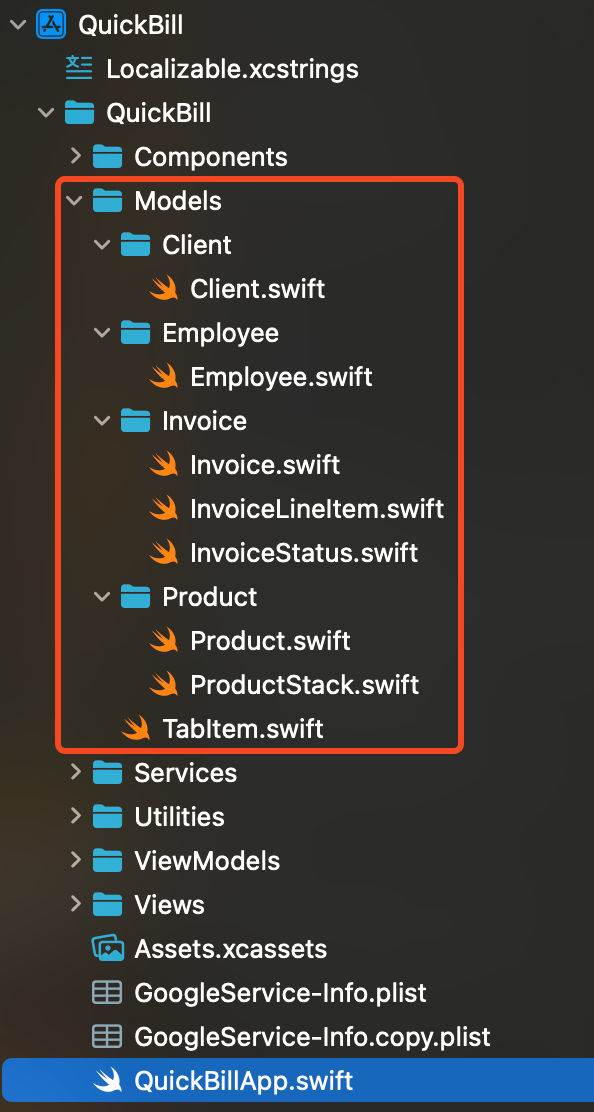
\includegraphics[width=0.5\textwidth]{Ilustraciones/ios_models_folder.png}
\caption{Estructura de la carpeta \texttt{Models} en Xcode}
\label{fig:models_folder}
\end{figure}

A continuación se describe brevemente el propósito de cada grupo.

\texttt{Models} agrupa todas las entidades que reflejan los documentos de Firestore. Cada subcarpeta contiene un único fichero con la estructura correspondiente:
\begin{itemize}
  \item \textbf{Client/Client.swift}: define la estructura \texttt{Client} con campos básicos de la empresa o persona a facturar.
  \item \textbf{Employee/Employee.swift}: representa a cada empleado que accede a la app. Incluye su \texttt{userId} (Firebase Auth), nombre, email, teléfono y rol.
  \item \textbf{Invoice}:
    \begin{itemize}
      \item \texttt{Invoice.swift}: entidad principal con fechas, importes y referencias a cliente y empleado.
      \item \texttt{InvoiceLineItem.swift}: describe cada línea de producto/servicio dentro de una factura.
      \item \texttt{InvoiceStatus.swift}: \texttt{enum} con los estados \texttt{paid}, \texttt{pending} y \texttt{overdue}.
    \end{itemize}
  \item \textbf{Product}:
    \begin{itemize}
      \item \texttt{Product.swift}: catálogo de productos con descripción y precio unitario.
      \item \texttt{ProductStack.swift}: colección de productos que se añaden a una factura.
    \end{itemize}
  \item \texttt{TabItem.swift}: enumeración con los tabs de navegación de la app.
\end{itemize}

\texttt{Services} agrupa la lógica que no depende de la UI pero tampoco encaja como modelo puro:
\begin{itemize}
  \item \texttt{AuthService.swift}: envoltorio sencillo sobre Firebase Auth con la finalidad de persistir la sesión de los usuarios en la aplicación.
  \item \texttt{InvoicePDFBuilder.swift}: genera el PDF de una factura usando UIGraphicsPDFRenderer; recibe una instancia \texttt{Invoice} y devuelve la URL local del fichero.
  \item \texttt{InvoiceStatusService.swift}: actualiza el estado de una factura (\texttt{paid}, \texttt{pending}, \texttt{overdue}) según \texttt{issuedAt}, \texttt{dueDate} y el \texttt{status} almacenado.
\end{itemize}

\texttt{Utilities} contiene código de soporte reutilizable. Actualmente sólo incluye \texttt{AppLanguage.swift}, una enumeración para cambiar el idioma de la interfaz mediante la propiedad \texttt{@AppStorage('appLanguage')}.

\texttt{ViewModels} se divide en subcarpetas por dominio de negocio:
\begin{itemize}
  \item \textbf{Authentication}: gestiona el inicio de sesión, registro y la opción de 'ovidé mi contraseña'.
  \item \textbf{Clients}: gestión de listado, creación, borrado y edición de clientes.
  \item \textbf{Invoice}: \texttt{InvoiceListViewModel.swift}, \texttt{InvoiceDetailViewModel.swift} y \texttt{AddInvoiceViewModel.swift} para listar, mostrar los detalles y crear nuevas faturas.
  \item \textbf{Products}: ViewModel para el catálogo de productos.
  \item \textbf{Settings}: controla las preferencias de la app.
  \item Además, en la raíz de la carpeta está \texttt{AuthViewModel.swift}, que mantiene el estado global de autenticación y se inyecta como \texttt{EnvironmentObject}.
\end{itemize}

\texttt{Views} organiza las pantallas SwiftUI con la misma lógica de dominios:
\begin{itemize}
  \item \textbf{Authentication}: vistas de inicio de sesión y registro.
  \item \textbf{Clients}: lista de clientes y formulario de creación y edición.
  \item \textbf{Home}: vista inicial tras iniciar sesión (dashboard con todas las facturas).
  \item \textbf{Invoice}: formulario de creación y detalles de las facturas.
  \item \textbf{Products}: listado y formulario de productos.
  \item \textbf{Settings}: ajustes de idioma y cuenta.
  \item \texttt{MainTabView.swift}: barra de pestañas inferior que enlaza \textit{Home}, \textit{Products}, \textit{Invoice}, \textit{Clients}, y \textit{Settings}.
  \item \texttt{StartView.swift}: pantalla que decide si mostrar la vista de autenticación o el \texttt{MainTabView} según el estado de \texttt{AuthViewModel}.
\end{itemize}

Esta distribución favorece la separación de responsabilidades, donde los 
ViewModels actúan como enlace entre modelos y vistas, y cada conjunto de vistas se mantiene cohesionado dentro de su propio dominio y los modelos definen la estructura de los datos que se manejan.

\end{large}

\subsection{Generación de PDF y numeración de facturas}

\begin{large}

En el diseño original se consideró usar Cloud Functions para generar el PDF, pero para evitar costes adicionales se implementó en la app iOS. Se creó una función en el ViewModel de detalle o en un servicio dedicado:

\begin{verbatim}
import UIKit
import PDFKit

func generatePDF(for invoice: Invoice) -> URL? {
    let pageWidth: CGFloat = 595.2  // A4 ancho en puntos
    let pageHeight: CGFloat = 841.8 // A4 alto en puntos
    let pdfMetaData = [
        kCGPDFContextCreator: "QuickBill",
        kCGPDFContextAuthor: "QuickBillApp"
    ]
    let format = UIGraphicsPDFRendererFormat()
    format.documentInfo = pdfMetaData as [String: Any]

    let renderer = UIGraphicsPDFRenderer(bounds: CGRect(x: 0, y: 0, width: pageWidth, height: pageHeight), format: format)
    let data = renderer.pdfData { (context) in
        context.beginPage()
        
        // Ejemplo de dibujo de título y tabla básica
        let titleFont = UIFont.systemFont(ofSize: 24, weight: .bold)
        let textAttributes: [NSAttributedString.Key: Any] = [
            .font: titleFont,
            .foregroundColor: UIColor.black
        ]
        let title = "Factura \(invoice.id ?? "")"
        title.draw(at: CGPoint(x: 72, y: 72), withAttributes: textAttributes)
        
        // Aquí se añadirían más líneas de texto con subtotales, impuestos, etc.
        // ...
    }

    let documentsURL = FileManager.default.urls(for: .documentDirectory, in: .userDomainMask)[0]
    let pdfURL = documentsURL.appendingPathComponent("factura_\(invoice.id ?? \"\").pdf")
    
    do {
        try data.write(to: pdfURL)
        return pdfURL
    } catch {
        print("Error al guardar PDF: \(error.localizedDescription)")
        return nil
    }
}
\end{verbatim}

Para la numeración, se utilizó el identificador único que Firestore asigna al documento. Así, cada factura ya cuenta con un número único sin necesidad de mantener un contador manual.

\end{large}

\subsection{Autenticación y permisos}

\begin{large}

La app utiliza Firebase Authentication con correo y contraseña. En la pantalla de inicio de sesión:

\begin{verbatim}
import SwiftUI
import FirebaseAuth

struct LoginView: View {
    @State private var email: String = ""
    @State private var password: String = ""
    @State private var errorMessage: String?

    var body: some View {
        VStack(spacing: 16) {
            TextField("Correo electrónico", text: $email)
                .autocapitalization(.none)
                .keyboardType(.emailAddress)
                .padding()
                .background(Color(.secondarySystemBackground))
                .cornerRadius(8)
            SecureField("Contraseña", text: $password)
                .padding()
                .background(Color(.secondarySystemBackground))
                .cornerRadius(8)
            if let error = errorMessage {
                Text(error)
                    .foregroundColor(.red)
            }
            Button(action: signIn) {
                Text("Iniciar sesión")
                    .frame(maxWidth: .infinity)
                    .padding()
                    .background(Color.blue)
                    .foregroundColor(.white)
                    .cornerRadius(8)
            }
        }
        .padding()
    }

    func signIn() {
        Auth.auth().signIn(withEmail: email, password: password) { result, error in
            if let error = error {
                self.errorMessage = error.localizedDescription
            } else {
                // Guardar uid en AppStorage o pasar a vista principal
                // ...
            }
        }
    }
}
\end{verbatim}

Una vez autenticado, el \texttt{currentUser.uid} se utiliza en cada consulta para filtrar facturas del empleado correspondiente:

\begin{verbatim}
db.collection("businesses")
  .document(businessId)
  .collection("invoices")
  .whereField("employeeId", isEqualTo: Auth.auth().currentUser?.uid ?? "")
  .getDocuments { snapshot, error in
    // ...
}
\end{verbatim}

\end{large}

\subsection{UI/UX y pruebas en simulador}

\begin{large}

Para verificar que todo funciona, se realizaron pruebas manuales en el simulador de iOS:

\begin{itemize}
  \item Crear una nueva factura: abrir \texttt{InvoiceFormView}, rellenar campos, pulsar “Guardar” y comprobar que aparece en \texttt{InvoiceListView}.
  \item Editar estado de factura: marcar una factura pendiente como “Paid” y verificar que cambia su color (verde) en la lista.
  \item Generar PDF: pulsar “Generar PDF” en \texttt{InvoiceDetailView} y verificar que se guarda en la carpeta \emph{Documents} del simulador.
  \item Inicio de sesión: probar con credenciales correctas e incorrectas para validar la lógica de \texttt{Auth}.
\end{itemize}

A continuación se muestran algunas capturas de pantalla (omitidas aquí) que ilustran estos flujos.

\end{large}

%----------------------------------------------------------
\section{Implementación web}
%----------------------------------------------------------

\begin{large}

La parte web, aunque más ligera, ofrece tres funcionalidades clave: gráfica de pagos mensuales, listado de morosos y tabla con todas las facturas. A continuación se describe su estructura y lógica:

\end{large}

\subsection{Estructura general del proyecto}

\begin{large}

El repositorio para el portal web sigue la convención estándar de Astro:
\begin{itemize}
  \item \texttt{/src/pages}:
    \begin{itemize}
      \item \texttt{index.astro}: página principal que importa los tres componentes.
      \item \texttt{invoices.astro}: gestión de todas las facturas (tabla).
      \item \texttt{overdue.astro}: listado de clientes morosos.
      \item \texttt{chart.astro}: componente independiente para la gráfica mensual.
    \end{itemize}
  \item \texttt{/src/components}:
    \begin{itemize}
      \item \texttt{MoneyChart.astro}: renderiza la gráfica de barras usando \emph{lightweight-charts}.
      \item \texttt{OverdueList.astro}: muestra tarjetas con clientes morosos y sus importes.
      \item \texttt{InvoiceTable.astro}: tabla con todas las facturas (ID, cliente, importe, estado, fecha).
    \end{itemize}
  \item \texttt{/src/firebase}:
    \begin{itemize}
      \item \texttt{firebase.ts}: inicializa Firebase con la configuración y exporta instancias de \texttt{firestore} y \texttt{auth}.
      \item \texttt{invoiceService.ts}: funciones para leer y escribir facturas en Firestore.
    \end{itemize}
  \item \texttt{/src/styles}:
    \begin{itemize}
      \item \texttt{globals.css}: importa y personaliza TailwindCSS.
      \item \texttt{variables.css}: define paletas de color y tipografías.
    \end{itemize}
\end{itemize}

\end{large}

\subsection{Carga de datos y renderizado}

\begin{large}

Para obtener las facturas del negocio, \texttt{invoiceService.ts} expone:

\begin{verbatim}
import { firestore } from "./firebase";

export async function getInvoices(businessId) {
  const snapshot = await firestore
    .collection(`businesses/${businessId}/invoices`)
    .orderBy("issuedAt", "desc")
    .get();
  return snapshot.docs.map(doc => ({ id: doc.id, ...doc.data() }));
}
\end{verbatim}

En \texttt{InvoiceTable.astro} se utiliza:

\begin{verbatim}
---
import { getInvoices } from "../firebase/invoiceService";
const businessId = Astro.site.businessId;
const invoices = await getInvoices(businessId);
---
<table class="min-w-full bg-white">
  <thead>
    <tr>
      <th class="px-4 py-2">ID</th>
      <th class="px-4 py-2">Cliente</th>
      <th class="px-4 py-2">Importe</th>
      <th class="px-4 py-2">Estado</th>
      <th class="px-4 py-2">Fecha</th>
    </tr>
  </thead>
  <tbody class="text-center">
    {invoices.map(inv => (
      <tr class="border-t">
        <td class="px-4 py-2">{inv.id}</td>
        <td class="px-4 py-2">{inv.clientName}</td>
        <td class="px-4 py-2">{inv.totalAmount.toFixed(2)}</td>
        <td class="px-4 py-2">{inv.status}</td>
        <td class="px-4 py-2">{new Date(inv.issuedAt).toLocaleDateString()}</td>
      </tr>
    ))}
  </tbody>
</table>
\end{verbatim}

Para el listado de morosos, \texttt{OverdueList.astro} filtra facturas cuyo estado sea “Pending” u “Overdue” y agrupa por cliente.

En \texttt{MoneyChart.astro}, se transforma el array \texttt{invoices} en dos series (pagos y pendientes) para la librería de gráficas:

\begin{verbatim}
---
import { createChart, HistogramSeries } from "https://cdn.jsdelivr.net/npm/lightweight-charts@5.0.7/+esm";

const invoiceData = await getInvoices(businessId);

// Agregar lógica para agrupar por mes y separar pagos/pendientes
const monthly = {};
invoiceData.forEach(inv => {
  const [year, month] = new Date(inv.issuedAt).toISOString().split("T")[0].split("-");
  const key = `${year}-${month}`;
  if (!monthly[key]) monthly[key] = { paid: 0, pending: 0 };
  if (inv.status === "Paid") {
    monthly[key].paid += inv.totalAmount;
  } else {
    monthly[key].pending += inv.totalAmount;
  }
});

const pendingData = [];
const paidData = [];
const ms12h = 12 * 60 * 60 * 1000;
Object.keys(monthly).sort().forEach(key => {
  const [yy, mm] = key.split("-");
  const base = new Date(`${yy}-${mm}-01T00:00:00Z`).getTime() / 1000;
  pendingData.push({ time: base, value: monthly[key].pending, color: "#facc15" });
  paidData.push({ time: base + ms12h, value: monthly[key].paid, color: "#16a34a" });
});

const container = document.getElementById("moneyChart");
const chart = createChart(container, {
  layout: { background: { color: "white" }, textColor: "#374151" },
  height: 250,
  timeScale: { tickMarkFormatter: time => new Date(time * 1000).toLocaleString("default", { month: "short" }) }
});
const pendSeries = chart.addSeries(HistogramSeries, { color: "#facc15" });
const paySeries = chart.addSeries(HistogramSeries, { color: "#16a34a" });
pendSeries.setData(pendingData);
paySeries.setData(paidData);
chart.timeScale().fitContent();
---
<div id="moneyChart" class="w-full h-64"></div>
\end{verbatim}

\end{large}

\subsection{Estilos y responsive}

\begin{large}

Para la tabla de facturas y la lista de morosos, se usaron clases de TailwindCSS:

\begin{itemize}
  \item Tablas: \texttt{class="min-w-full bg-white"}, encabezados con \texttt{px-4 py-2 text-left font-medium}, filas con \texttt{border-t text-center}.
  \item Tarjetas de morosos: \texttt{class="bg-white shadow rounded p-4 hover:shadow-lg grid grid-cols-1 sm:grid-cols-2 md:grid-cols-3 gap-4"}.
  \item Gráfica: contenedor con \texttt{class="w-full h-64"} para acomodar el lienzo de \emph{lightweight-charts}.
\end{itemize}

La configuración responsive se logra con clases como \texttt{grid-cols-1 md:grid-cols-2 lg:grid-cols-3} y utilidades de Tailwind para márgenes y paddings en distintos puntos de ruptura.

\end{large}

\subsection{Despliegue del portal en Vercel}

\begin{large}
	
El portal web se despliega en Vercel siguiendo el flujo de integración continua:

\begin{enumerate}
  \item Cada vez que se hace \emph{push} a la rama \texttt{main}, Vercel detecta el cambio y ejecuta el comando \texttt{npm run build}.
  \item Una vez compilado, Vercel optimiza los activos estáticos y publica el sitio en una URL de producción.
  \item Se configuró un dominio personalizado y se activaron los certificados TLS automáticos.
\end{enumerate}

A continuación se muestra una captura del panel de Vercel donde se observa el estado del último despliegue y la URL asignada (omitida en este texto).

\end{large}